\section{La constante de la circunferencia} % (fold)
\label{sec:the_circle_constant}

\href{http://tauday.com/tau-manifesto}{\emph{El manifiesto tau}} está dedicado a uno de los números más importantes en matemáticas, quizá \emph{el más} importante: la \emph{constante de la circunferencia}, que relaciona su perímetro con su dimensión lineal. Desde hace miles de años, la circunferencia se ha considerado la más perfecta de todas las formas, y su constante captura su geometría en un único número. Desde luego, la elección tradicional para la constante de la circunferencia es $\pi$---pero, como señala el matemático \href{http://www.math.utah.edu/~palais}{Bob Palais} en su delicioso artículo ``$\pi$ Is Wrong!'',\footnote{Palais, Robert. ``$\pi$ Is Wrong!'', \emph{The Mathematical Intelligencer}, Volumen~23, Número~3, 2001, pp.~7--8. Muchos de los alegatos de \emph{El manifiesto tau} están basados en, o inspirados por, ``$\pi$ Is Wrong!''. Está disponible online en \href{http://www.math.utah.edu/~palais/pi.html}{http://bit.ly/pi-is-wrong}.} $\pi$ \emph{está mal}. Es hora de hacer justicia.

  \subsection{Una propuesta poco modesta} % (fold)
  \label{sec:an_immodest_proposal}

Comencemos a reparar el daño causado por $\pi$ comprendiendo en primer lugar el famoso número en sí. La definición tradicional para la constante de la circunferencia define $\pi$ (pi) como la razón entre el perímetro de una circunferencia y su diámetro:\footnote{El símbolo $\equiv$ significa ``se define como''.}
\begin{equation}
\label{eq:pi}
\pi \equiv \frac{C}{D} = 3.14159265\ldots
\end{equation}
El número $\pi$ tiene muchas propiedades notables ---entre otras cosas, es un número \href{https://es.wikipedia.org/wiki/Número_irracional}{\emph{irracional}} y de hecho \href{https://es.wikipedia.org/wiki/Número_trascendente}{\emph{trascendente}}--- y aparece por doquier en fórmulas matemáticas.

\begin{figure}
\image{images/figures/circle.pdf}
\caption{Anatomía de una circunferencia.\label{fig:circle}}
\end{figure}
%TODO Traducir esta imagen

Debería resultar obvio que $\pi$ no está ``mal'' en el sentido de ser factualmente incorrecto; el número $\pi$ está perfectamente bien definido, y posee todas las propiedades que los matemáticos habitualmente le atribuyen. Cuando decimos que ``$\pi$ está mal'', queremos decir que \emph{$\pi$ es una elección confusa y poco natural para la constante de la circunferencia}. En particular, una circunferencia se define como el lugar geométrico de los puntos de un plano que se encuentran a una distancia fija ---el \emph{radio}--- de un punto dado, el \emph{centro} (Figure~\ref{fig:circle}). Así como hay infinitas formas con diámetro constante (figura~\ref{fig:bicycle_constant_diameters}), solo hay una forma que tenga radio constante. Esto parece sugerir que una definición más natural para la constante de la circunferencia podría utilizar $r$ en lugar de $D$:
\begin{equation}
\label{eq:circle_constant}
\mbox{constante de la circunferencia} \equiv \frac{C}{r}.
\end{equation}
Como el diámetro de una circunferencia es el doble que su radio, este número es igual a $2\pi$. Como $\pi$, es transcendente y por tanto irracional, y (como veremos en la sección~\ref{sec:the_number_tau}) su uso en matemáticas está igualmente extendido.

\begin{figure}
\image{images/figures/bicycle_constant_diameters.png}
\caption{Dos de las infinitas posibles formas con diámetro constante.\label{fig:bicycle_constant_diameters}}
\end{figure}

En ``$\pi$ Is Wrong!'', Bob Palais argumenta persuasivamente a favor de la segunda de estas dos definiciones de la constante del círculo, y desde mi punto de vista él merece 
todo el reconocimiento por haber identificado el problema y haberlo hecho llegar a un amplio público. Él denominó a la verdadera constante de la circunfencia ``una vuelta'', y también introdujo un nuevo símbolo para representarla (figura~\ref{fig:palais_tau}). Como veremos, su descripción es clarividente, pero desafortunadamente el símbolo es más bien raro, y (como se discute en la sección~\ref{sec:conflict_and_resistance}) parece poco probable que pueda ser adoptado de manera generalizada.

\begin{figure}
\imagebox{images/figures/palais-tau.png}
\caption{El extraño símbolo para la constante de la circunferencia de ``$\pi$ Is Wrong!''.\label{fig:palais_tau}}
\end{figure}

\emph{El manifiesto tau} está dedicado a exponer que la respuesta correcta a ``$\pi$ está mal'' es ``no, \emph{en serio}''; y a que la verdadera constante de la circunferencia merece un nombre adecuado. Como ya habrás podido suponer, \emph{El manifiesto tau} propone que ese nombre sea la letra griega $\tau$ (tau):
\begin{equation}
\label{eq:tau}
\tau \equiv \frac{C}{r} = 6.283185307179586\ldots
\end{equation}
A lo largo del resto de este manifiesto, veremos que el \emph{número} $\tau$ es la elección correcta, y trataremos de mostrar a través del uso (sección~\ref{sec:the_number_tau} y sección~\ref{sec:circular_area}) y de manera directa, mediante argumentación, (sección~\ref{sec:conflict_and_resistance}) que la  \emph{letra} $\tau$ también es una elección natural.

\subsection{Un poderoso enemigo} % (fold)
 \label{sec:a_powerful_enemy}

Antes de comenzar a demostrar que $\tau$ es la elección natural para la constante de la circunferencia, reconozcamos antes a quién nos enfrentamos ---y es que hay una poderosa conspiración, desde hace cientos de años, decidida a propagar propaganda pro-$\pi$. Se  \href{http://www.amazon.com/exec/obidos/ISBN=0802713327/parallaxproductiA/}{escriben} \href{http://www.amazon.com/Pi-Sky-Counting-Thinking-Being/dp/0198539568}{libros} \href{http://www.amazon.com/exec/obidos/ISBN=0312381859/parallaxproductiA/}{enteros} alabando las virtudes de $\pi$ (o sea, ¡\href{http://www.amazon.com/exec/obidos/ISBN=0387989463/parallaxproductiA/}{\emph{libros}}!). Y la devoción irracional por  $\pi$ se ha extendido hasta los más altos niveles de frikismo; por ejemplo, en el ``día de pi'' de 2010, \href{http://www.google.com/}{Google} \emph{cambió su logo} en honor de $\pi$  (Figure~\ref{fig:google_pi_day.}).
%TODO Buscar versiones en castellano de estos enlaces

\begin{figure}
\begin{center}
\image{images/figures/google_pi_day.png}
\end{center}
\caption{El logo de Google el día 14 de marzo (3/14, en notación inglesa) de 2010, (el ``día de pi'').\label{fig:google_pi_day.}}
\end{figure}

Mientras tanto, hay personas que memorizan docenas, cientos o incluso  \href{https://en.wikipedia.org/wiki/Lu_Chao}{\emph{miles}} de dígitos de este número místico. ¿Que clase de patética persona memoriza siquiera 40 dígitos de $\pi$ (figura~\ref{fig:futurama_video})?\footnote{El vídeo en la figura~\ref{fig:futurama_video} (disponible en  \href{http://vimeo.com/12914981}{http://vimeo.com/12914981}) es un extracto de una clase impartida por la \href{http://mathsci.appstate.edu/~sjg/}{Dra.\ Sarah Greenwald}, profesora de matemáticas en la \href{http://www.appstate.edu/}{Appalachian State University}. La doctora\ Greenwald utiliza referencias de matemáticas de  \emph{Los Simpsons} y \emph{Futurama} para captar la atención de sus estudiantes y para ayudarles a superar su miedo hacia las matemáticas. Además, mantiene la \href{http://mathsci2.appstate.edu/~sjg/futurama/}{\emph{Futurama} Math Page}.}
%TODO Traducir Futurama Math Page? Mismo criterio que con pi is wrong, etc.

\begin{figure}
\begin{center}
%= insert_futurama_video
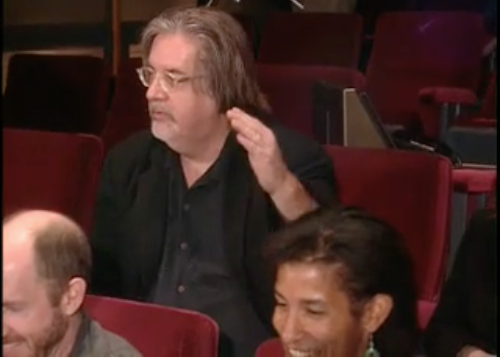
\includegraphics{images/figures/futurama_math_lecture.png} % html_ignore
\end{center}
\caption{\href{https://tauday.com/tau-manifesto/\#sec-about_the_author}{Michael Hartl} demuestra que \href{https://en.wikipedia.org/wiki/Matt_Groening}{Matt Groening} se equivoca recitando 40 dígitos decimales de $\pi$.\label{fig:futurama_video}}
\end{figure}

En verdad, las personas partidarias de $\tau$ nos enfrentamos a un imponente adversario. Y sin embargo, contamos con una poderosa aliada ---pues la verdad está de nuestra parte.

% section the_most_important_number (end)

\section{El número tau} % (fold)
\label{sec:the_number_tau}

En la sección~\ref{sec:an_immodest_proposal} vimos que el número $\tau$ se puede escribir también como $2\pi$. Por tanto, como se señala en ``$\pi$ Is Wrong!'', resulta de gran interés descubrir que la combinación $2\pi$ se encuentra con asombrosa frecuencia en todas las ramas de las matemáticas. Considérense, por ejemplo, las integrales espaciales en coordenadas polares:
\[
  \int_0^{2\pi}\int_0^\infty f(r, \theta)\, r\, dr\, d\theta.
\]
El límite superior de integración de la variable $\theta$ siempre es $2\pi$. Aparece el mismo factor en la definición de la \href{https://es.wikipedia.org/wiki/Distribución_normal}{distribución gaussiana (normal)},
\[
  \frac{1}{\sqrt{2\pi}\sigma}e^{-\frac{(x-\mu)^2}{2\sigma^2}},
\]
y, nuevamente, en la  \href{http://mathworld.wolfram.com/FourierTransform.html}{transformada de Fourier},
\[
  f(x) = \int_{-\infty}^\infty F(k)\, e^{2\pi ikx}\,dk
\]
\[
    F(k) = \int_{-\infty}^\infty f(x)\, e^{-2\pi ikx}\,dx.
\]
Reaparece también en la \href{https://es.wikipedia.org/wiki/Fórmula_integral_de_Cauchy}{fórmula integral de Cauchy},
\[
  f(a) = \frac{1}{2\pi i}\oint_\gamma\frac{f(z)}{z-a}\,dz,
\]
en las $n$th \href{https://es.wikipedia.org/wiki/Raíz_de_la_unidad}{raíces de la unidad},
\[
  z^n = 1 \Rightarrow z = e^{2\pi i/n},
\]
y en los valores de la \href{https://es.wikipedia.org/wiki/Función_zeta_de_Riemann}{función zeta de Riemann} para enteros positivos pares:\footnote{Aquí $B_n$ es el $n$-ésimo \href{https://es.wikipedia.org/wiki/Número_de_Bernoulli}{número de Bernoulli}.}
\[
  \zeta(2n) = \sum_{k=1}^\infty \frac{1}{k^{2n}} = \frac{B_n}{2(2n)!}\,(2\pi)^{2n}.\qquad n = 1, 2, 3, \ldots
\]
Estas fórmulas no están elegidas a propósito ---abre por cualquier página tu libro favorito de física o matemáticas y compruébalo por ti mismo. Hay  \href{http://www.harremoes.dk/Peter/Undervis/Turnpage/Turnpage1.html}{muchos más ejemplos}, pero en todo caso la conclusión está clara: $2\pi$~es especial.
%TODO Elegir entre tú y usted

Para llegar al fondo de este misterio, debemos volver a los fundamentos y analizar la naturaleza de las circunferencias, y especialmente la naturaleza de los \emph{ángulos}. Aunque es probable que la mayor parte de este material resultará familiar, merece la pena volver a verlo, ya que es aquí donde comienza la auténtica comprensión de $\tau$.

  \subsection{Circunferencias y ángulos} % (fold)
  \label{sec:circles_and_angles}

Existe una estrecha relación entre las circunferencias y los ángulos, tal y como muestra la figura~\ref{fig:angle_arclength}. Como las circunferencias concéntricas en la figura~\ref{fig:angle_arclength} tienen radios difrentes, las líneas del dibujo cortan distintas \emph{longitudes de arcoarc lengths}, pero el ángulo~$\theta$ (theta) es el mismo en ambos casos. En otras palabras, el tamaño de los ángulos no depende del radio de la circunferencia empleada para definir el arco. La tarea principal de la medida de ángulos es crear un sistema que capte esta invarianza respecto al radio.

\begin{figure}
\begin{center}
\image{images/figures/angle-arclength.pdf}
\end{center}
\caption{Un ángulo $\theta$ con dos circunferencias concéntricas.\label{fig:angle_arclength}}
\end{figure}

Quizá el sistema de ángulos más rudimentario es el basado en  \emph{grados}, que divide una circunferencia en 360 partes iguales. Una resultado de este sistema es el conjunto de ángulos especiales (familiares para quienes estudian trigonometría) que muestra la figura~\ref{fig:degree_angles}.

\begin{figure}
\begin{center}
\image{images/figures/degree-angles.pdf}
\end{center}
\caption{Algunos ángulos especiales, en grados.\label{fig:degree_angles}}
\end{figure}

Un sistema más fundamental de medida de ángulos requiere una comparación directa entre la longitud de arco $s$ y el radio $r$. Aunque las longitudes de la figura~\ref{fig:angle_arclength} son diferentes, la longitud de arco crece en proporción al radio, de manera que el \emph{cociente} entre la longitud de arco y el radio es el mismo en ambos casos:
\[
s\propto r \Rightarrow \frac{s_1}{r_1} = \frac{s_2}{r_2}.
\]
Esto sugiere la siguiente definición de  \emph{medida de ángulos en radianes}:
\begin{equation}
\label{eq:radians}
\theta \equiv \frac{s}{r}.
\end{equation}
Esta definición posee la propiedad requerida de ser invariante con respecto al radio, y dado que tanto  $s$ como $r$ tienen unidades de longitud, los radianes son  \href{https://es.wikipedia.org/wiki/Magnitud_adimensional}{\emph{adimensionales}} por construcción. Medir ángulos en radianes da lugar a fórmulas concisas y elegantes en matemáticas; por ejemplo, la fórmula habitual para la derivada de  $\sin\theta$ es cierta solamente cuando  $\theta$ se expresa en radianes:
\[
  \frac{d}{d\theta}\sin\theta = \cos\theta. \qquad\mbox{(true only when $\theta$ is in radians)}
\]
Naturalmente, los ángulos especiales de la figura~\ref{fig:degree_angles} se pueden expresar en radianes, y cuando aprendiste trigonometría en secundaria probablemente tuviste que memorizar los valores especiales que se muestran en la figura~\ref{fig:pi_angles} (denomino a esta unidad de medida $\pi$-radián para enfatizar que están escritos en términos de $\pi$).

\begin{figure}
\begin{center}
\image{images/figures/pi-angles.pdf}
\end{center}
\caption{Algunos ángulos especiales, en $\pi$-radianes.\label{fig:pi_angles}}
\end{figure}

\begin{figure}
\begin{center}
\image{images/figures/angle-fractions.pdf}
\end{center}
\caption{Los ángulos ``especiales'' son fracciones de una circunferencia completa.\label{fig:angle_fractions}}
\end{figure}

Si lo pensamos por un momento, vemos que estos ángulos ``especiales'' no son más que  \emph{fracciones racionales} particularmente sencillas de una circunferencia completa, como se muestra en la figura~\ref{fig:angle_fractions}. Esto invita a revisar la ecuación~\eqref{eq:radians}, reescribiendo la longitud de arco~$s$ en función de la fracción~$f$ de la circunferencia completa~$C$, i.e., $s = f C$:
\[ \theta = \frac{s}{r} = \frac{fC}{r} =  f\left(\frac{C}{r}\right) \equiv f\tau. \]
Nótese cuán naturalmente se desprende $\tau$ de este análisis. Si eres una persona creyente en $\pi$, me temo que el diagrama resultante de ángulos especiales (figura~\ref{fig:tau_angles}) sacudirá tu fe desde sus entrañas.

\begin{figure}
\begin{center}
\image{images/figures/tau-angles.pdf}
\end{center}
\caption{Algunos ángulos especiales, en radianes.\label{fig:tau_angles}}
\end{figure}

Aunque hay muchos otros argumentos a favor de $\tau$, puede que la figura~\ref{fig:tau_angles} sea el más sorprendente. En la figura~\ref{fig:tau_angles} vemos también el genio de la identificación que hizo Bob Palais de la constante de la circunferencia como ``\href{https://en.wikipedia.org/wiki/Turn_(geometry)}{una vuelta}'':
%TODO No hay versión en castellano
 $\tau$ es la medida de ángulo en radianes para una \emph{vuelta} de circunferencia. Es más: nótese que con $\tau$ \emph{no hay nada que memorizar}: la duodécima parte de una vuelta es $\tau/12$, la octava parte de una vuelta es $\tau/8$, y así sucesivamente. Utilizar $\tau$ nos da lo mejor de ambos mundos, combinando claridad conceptual con todos los beneficios específicos de los radianes; el significado abstracto de, por ejemplo, $\tau/12$ es obvio, pero también es simplemente un número:
\[
  \mbox{la duodécima parte de una vuelta} = \frac{\tau}{12} \approx \frac{6.283185}{12} = 0.5235988.
\]
Por último, si comparamos la figura~\ref{fig:pi_angles} con la figura~\ref{fig:tau_angles}, vemos de dónde proceden esos engorrosos factores de $2\pi$: una vuelta de circunferencia es $1\tau$, pero $2\pi$. Numéricamente son iguales, pero conceptualmente son bien distintos.

    \subsubsection{Las repercusiones} % (fold)
    \label{sec:the_ramifications}
%TODO The ramifications: revisar esta traducción
    % subsubsection the_ramifications (end)

Esos innecesarios factores de $2$ que se derivan del uso de $\pi$ son suficientemente molestos por sí mismos, pero más grave aún es su tendencia a cancelarse cuando se dividen por cualquier número par. Se producen resultados absurdos, como la  \emph{mitad} de $\pi$ para un \emph{cuarto} de vuelta, que ocultan la relación subyacente entre la medida de un angulo y la constante de la circunferencia. A quienes sostienen que ``da igual'' utilizar $\pi$ o $\tau$ al enseñar trigonometría solo les pido per vean la figura~\ref{fig:pi_angles}, la figura~\ref{fig:angle_fractions} y la figura~\ref{fig:tau_angles} a través de los ojos de un niño o niña. Verán que, desde la perspectiva de quien empieza a aprender, \href{http://tauday.com/a-tau-testimonial}{\emph{usar $\pi$ en lugar de $\tau$ es un desastre pedagógico}}.

  \subsection{Las funciones circulares} % (fold)
  \label{sec:the_circle_functions}

%TODO Hay que modificar sin para que se genere como sen. También en las gráficas
Aunque la medida de ángulos en radianes ofrece algunos de los argumentos más convincentes acerca de la constante de la circunferencia, también vale la pena comparar las virtudes de $\pi$ y $\tau$ en otros contextos. Empecemos por considerar las importantes funciones básicas $\sin\theta$ y $\cos\theta$. Conocidas como ``funciones circulares'' por dar las coordenadas de un punto en la \emph{circunferencia unitaria} (i.e., una circunferencia con radio~$1$), el seno y el coseno son funciones fundamentales en trigonometría (figura~\ref{fig:circle_functions}).

%TODO Traducir esta imagen
\begin{figure}
\begin{center}
\image{images/figures/circle-functions.pdf}
\end{center}
\caption{Las funciones circulares son coordenadas en la circunferencia unitaria.\label{fig:circle_functions}}
\end{figure}

Examinemos las gráficas de las funciones circulares para comprender mejor su comportamiento.\footnote{Estas gráficas se han generado con la ayuda de \href{http://www.wolframalpha.com/}{Wolfram|Alpha}.} En la figura ~\ref{fig:sine_with_tau} y la figura~\ref{fig:cosine_with_tau} se observa que ambas funciones son \emph{periódicas} con periodo $T$. Como se muestra en la figura~\ref{fig:sine_with_tau}, la función $\sin\theta$ comienza en cero, alcanza un máximo al llegar a un cuarto del periodo, pasa por cero en la mitad del periodo, alcanza un mínimo en las tres cuartas partes del periodo y vuelve a cero tras un periodo completo. Por su parte, la función $\cos\theta$ comienza en un máximo, tiene un mínimo en la mitad del periodo y pasa por cero en un cuarto y tres cuartos del periodo (figura~\ref{fig:cosine_with_tau}). A modo de referencia, ambas figuras muestran el valor de $\theta$ (en radianes) en cada punto especial.

\begin{figure}
\begin{center}
\image{images/figures/sine-with-tau.pdf}
\end{center}
\caption{Puntos importantes de $\sin\theta$ en relación con el periodo $T$.\label{fig:sine_with_tau}}
\end{figure}

\begin{figure}
\begin{center}
\image{images/figures/cosine-with-tau.pdf}
\end{center}
\caption{Puntos importantes de $\cos\theta$ en relación con el periodo $T$.\label{fig:cosine_with_tau}}
\end{figure}

%TODO Plantear si traducir i.e. por algo más coloquial en castellano (como "es decir")
Por supuesto, dado que tanto seno como coseno completan una ciclo completo durante una vuelta alrededor de la circunferencia, tenemos que $T = \tau$; es decir, las funciones circulares tienen periodos iguales a la constante de la circunferencia. Como consecuencia, los valores ``especiales''de $\theta$ son completamente naturales: un cuarto del periodo es $\tau/4$, la mitad del periodo es $\tau/2$, etc. De hecho, al generar la figura~\ref{fig:sine_with_tau}, me encontré en un momento dado pensando en cuál sería el valor numérico de $\theta$ para el cero de la función seno. Dado que el cero se produce tras medio periodo, y dado que $\tau \approx 6.28$, un cálculo mental rápido me condujo al siguiente resultado:
\[
  \theta_\mathrm{cero} = \frac{\tau}{2} \approx 3.14.
\]
Así es: me quedé atónito al descubrir que \emph{ya había olvidado que a veces $\tau/2$ se llama ``$\pi$''.} Quizá incluso te acaba de pasar lo mismo a ti. Bienvenido a mi mundo.

  % subsection the_circle_functions (end)

% section radian_angle_measure (end)

   \subsection{La identidad de Euler} % (fold)
   \label{sec:euler_s_identity}

Sería un descuido por mi parte no atender a la \emph{identidad de Euler}, algunas veces calificada como ``la ecuación más hermosa en matemáticas''. Esta identidad involucra a la \emph{exponencial compleja}, que está profundamentamente conectada tanto con la constante de la circunferencia como con su misma geometría.

Dependiendo del camino elegido, la siguiente ecuación se puede demostrar como teorema o tomar como definición; en cualquier caso, es realmente excepcional:
\begin{equation}
\label{eq:eulers_formula}
e^{i\theta} = \cos\theta + i\sin\theta. \qquad\mbox{Fórmula de Euler}
\end{equation}
Conocida como la \emph{fórmula de Euler} (en honor a \href{https://en.wikipedia.org/wiki/Leonhard_Euler}{Leonhard Euler}), esta ecuación relaciona una exponencial con argumento imaginario con las funciones circulares seno y coseno y con la unidad imaginaria~$i$. Aunque explicar la fórmula de Euler queda fuera del alcance de este manifiesto, su procedencia no es precisamente sospechosa, y su importancia es incuestionable.

Evaluar la ecuación~\eqref{eq:eulers_formula} en $\theta = \tau$ produce la \emph{identidad de Euler}:\footnote{Aquí estoy difiniendo implícitamente la identidad de Euler como la \emph{exponencial compleja de la constante de la circunferencia} en lugar de definirla como la exponencial compleja de cualquier número en particular. Si elegimos  $\tau$ como la constante de la circunferencia, obtenemos la identidad mostrada. Como veremos en breve, esta no es la forma tradicional de la identidad, que por supuesto involucra a $\pi$, pero la versión con  $\tau$ es la forma más  \emph{matemáticamente}significativa de la identidad, así que creo que merece el nombre.}
\[ e^{i\tau} = 1. \qquad\mbox{Identidad de Euler (versión con $\tau$)} \]
Expresado en palabras, esta ecuación realiza la siguiente observación fundamental:

\begin{center}
\emph{La exponencial compleja de la constante de la circunferencia es la unidad.}
\end{center}

Geométricamente, multiplicar por $e^{i\theta}$ equivale a rotar un número complejo un ángulo $\theta$ en el plano complejo, lo que sugiere una segunda interpretación de la identidad de Euler:

\begin{center}
\emph{Una rotación de una vuelta es 1.}
\end{center}

%TODO revisar si todos los enlaces de wikipedia están cambiados por su versión castellana
\noindent Dado que el número $1$ es la \href{https://es.wikipedia.org/wiki/Elemento_neutro}{identidad multiplicativa}, el significado geométrico de $e^{i\tau} = 1$ es que rotar un punto en el plano complejo una vuelta completa simplemente lo devuelve a su posición original.

Como en el caso de la medida de ángulos en radianes, vemos cuán natural es la asociación entre $\tau$ y una vuelta alrededor de una circunferencia. Tanto es así, que la identificación de $\tau$ con ``una vuelta'' hace que la identidad de Euler suene cai como una tautología.\footnote{Técnicamente, todos los teoremas matemáticos son tautologías, pero no seamos tan pedantes.}

%TODO Uf, este título suena rarísimo
    \subsubsection{No la ecuación más hermosa} % (fold)
    \label{sec:not_the_most_beautiful_equation}

Por supuesto, la forma tradicional de la ecuación de Euler se escribe en término de $\pi$ en lugar de $\tau$. Para obtenerla, comenzamos por evaluar la fórmula de Euler en $\theta = \pi$, lo que produce
\begin{equation}
\label{eq:eulers_identity_pi}
e^{i\pi} = -1. \qquad\mbox{Identidad de Euler (versión con $\pi$)}
\end{equation}
Pero ese signo menos es tan feo que la fórmula casi siempre se reordena inmediatamente, produciendo la siguiente ``hermosa'' ecuación:
\[ e^{i\pi} + 1 = 0. \qquad\mbox{Identidad de Euler (reordenada)} \]
Al llegar a este punto, habitualmente quien explica realiza una afirmación grandilocuente sobre cómo la identidad de Euler relaciona $0$, $1$, $e$, $i$ y $\pi$ ---en ocasiones llamados los ``cinco números más importantes en matemáticas''. Es impresionante la cantidad de gente que se queja de que la identidad de Euler con $\tau$ solo relaciona \emph{cuatro} de estos cinco. De acuerdo:
\[ e^{i\tau} = 1 + 0. \]
Esta fórmula, \emph{sin} reordenar, en relaciona verdaderamente los cinco números más imporantes en matemáticas: $0$, $1$, $e$, $i$ y $\tau$.

      \subsubsection{Identidades eulerianas} % (fold)
      \label{sec:eulerian_identities}

Dado que es posible añadir cero en cualquier ecuación, introducir $0$ en la fórmula $e^{i\tau} = 1 + 0$ no deja de ser un contrapunto irónico de $e^{i\pi} + 1 = 0$, pero realmente puede extraerse algo importante de la identidad $e^{i\pi} = -1$. Veamos qué sucede cuando la reescribimos en términos de $\tau$:
%TODO en términos de.
\[
e^{i\tau/2} = -1.
\]
Geométricametne, esto significa que una rotación de media vuelta es lo mismo que multiplicar por $-1$. Y efectivamente, así es: tras una rotación de $\tau/2$ radianes, el número complejo $z = a + ib$ queda asignado a $-a - ib$, que es de hecho $-1\cdot z$.

Escrita en términos de $\tau$, vemos que la forma ``original'' de la identidad de Euler (ecuación~\eqref{eq:eulers_identity_pi}) tiene un significado geométrico obvio del que carece cuando se escribe en términos de $\pi$ (por supuesto, $e^{i\pi} = -1$ se puede interpretar como una rotación por $\pi$ radianes, pero la casi universal reordenación a la forma $e^{i\pi} + 1 = 0$ evidencia cómo el uso de $\pi$ desvía la atención del significado geométrico natural de la identidad). Las identidades de un cuarto de ángulo tienen interpretaciones geométricas similares: evaluar la ecuación~\eqref{eq:eulers_formula} en $\tau/4$ nos da $e^{i\tau/4} = i$, que significa que un cuarto de vuelta en el plano complejo es lo mismo que multiplicar por~$i$; igualmente, $e^{i\cdot(3\tau/4)} = -i$ quiere decir que tres cuartos de vuelta es lo mismo que multiplicar por~$-i$. Un resumen de estos resultados, que denominaremos \emph{identidades eulerianas}, se presenta en la tabla~\ref{table:eulerian_identities}.
%TODO revisar puntos dentro de, o antes de, paréntesis

\begin{table}
\begin{center}
\begin{tabular}{cllr}
Ángulo de rotación & \multicolumn{3}{c}{Identidad euleriana} \\ \hline
$0$ & $e^{i\cdot0}$ & $ = $ & $1$ \smallskip \\
$\tau/4$ & $e^{i\tau/4}$ & $ = $ & $i$ \smallskip \\
$\tau/2$ & $e^{i\tau/2}$ & $ = $ & $-1$ \smallskip \\
$3\tau/4$ & $e^{i\cdot(3\tau/4)}$ & $ = $ & $-i$ \smallskip \\
$\tau$ & $e^{i\tau}$ & $ = $ & $1$
\end{tabular}
\end{center}
\caption{Identidades eulerianas para rotaciones de media vuelta, cuartos y completa.\label{table:eulerian_identities}}
\end{table}

Podemos llevar este análisis un paso más allá señalando que, para cualquier ángulo~$\theta$, se puede interpretar $e^{i\theta}$ como un punto perteneciente a la circunferencia unidad en el plano complejo. Como el plano complejo identifica el eje horizontal con la parte real del número y el eje vertical con la parte imaginaria, la fórmula de Euler nos dice que $e^{i\theta}$ son las coordenadas $(\cos\theta, \sin\theta)$. Introducir los valores de los ángulos ``especiales'' de la figura~\ref{fig:tau_angles} en la ecuación~\eqref{eq:eulers_formula} nos da entonces los puntos de la tabla~\ref{table:complex_exponentials}, y dibujar estos puntos en el plano complejo produce la figura~\ref{fig:tau_euler_circle}. Una comparativa entre la figura~\ref{fig:tau_euler_circle} y la figura~\ref{fig:tau_angles} disipa rápidamente cualquier duda acerca de cuál de las constantes de la circunferencia revela mejor la relación entre la fórmula de Euler y la geometría del círculo.
%TODO ver si compensa abreviar ecuación~

\begin{table}
\begin{center}
\begin{tabular}{lcc}
Forma polar & Forma rectangular & Coordenadas \\ \hline\hline
$e^{i\theta}$ & $\cos\theta + i\sin\theta$ & $(\cos\theta, \sin\theta)$ \\ \hline
$e^{i\cdot0}$ & $1$ & $(1, 0)$ \smallskip \\
$e^{i\tau/12}$ & $\frac{\sqrt{3}}{2} + \frac{1}{2}i$ & $(\frac{\sqrt{3}}{2}, \frac{1}{2})$ \smallskip \\
$e^{i\tau/8}$ & $\frac{1}{\sqrt{2}} +  \frac{1}{\sqrt{2}}i$ & $(\frac{1}{\sqrt{2}}, \frac{1}{\sqrt{2}})$ \smallskip \\
$e^{i\tau/6}$ & $\frac{1}{2} +\frac{\sqrt{3}}{2} i$ & $(\frac{1}{2}, \frac{\sqrt{3}}{2})$ \smallskip \\
$e^{i\tau/4}$ & $i$ & $(0, 1)$ \smallskip \\
$e^{i\tau/3}$ & $-\frac{1}{2} +\frac{\sqrt{3}}{2} i$ & $(-\frac{1}{2}, \frac{\sqrt{3}}{2})$ \smallskip \\
$e^{i\tau/2}$ & $-1$ & $(-1, 0)$ \smallskip \\
$e^{i\cdot(3\tau/4)}$ & $-i$ & $(0, -1)$ \smallskip \\
$e^{i\tau}$ & $1$ & $(1, 0)$
\end{tabular}
\end{center}
\caption{Exponenciales complejas de los ángulos especiales de la figura~\ref{fig:tau_angles}.\label{table:complex_exponentials}}
\end{table}

\begin{figure}
\begin{center}
\image{images/figures/tau_euler_circle.pdf}
\end{center}
\caption{Exponenciales complejas de algunos ángulos especiales dibujados en el plano complejo.\label{fig:tau_euler_circle}}
\end{figure}
%TODO Traducir todos los "Table" y "Figure" de los caption. spanish babel?

      % subsubsection eulerian_identities (end)

\section{El área del círculo: el \emph{golpe de gracia}} % (fold)
\label{sec:circular_area}

%TODO repasar estos guiones y contrastar con el original
Si has llegado aquí como un creyente en $\pi$, a estas alturas deberías estar cuestionando tu fe. $\tau$ es tan natural, su significado tan obvio... ¿No hay ningún ejemplo en que $\pi$ brille con toda su gloria? Se agita un recuerdo ---sí, existe una fórmula así---, ¡es la fórmula del área del círculo! Contemplad:
\[ A = \tfrac{1}{4} \pi D^2. \]
No, un momento. La fórmula del área se escribe siempre en términos del \emph{radio}, de la siguiente manera:
\[ A = \pi r^2. \]
Aquí vemos a$\pi$, sin adornos, en una de las ecuaciones más importantes en matemáticas ---una fórmula demostrada por primera vez por el mismísimo \href{https://es.wikipedia.org/wiki/Arquímedes}{Arquímedes}. ¡Queda reestablecido el orden! Y sin embargo, el nombre de esta sección suena inquietante\ldots\ Si esta ecuación es la gloriosa coronación de $\pi$, ¿cómo puede ser también su \href{https://es.wikipedia.org/wiki/Tiro_de_gracia}{\emph{golpe de gracia}}?


  \subsection{Formas cuadráticas} % (fold)
  \label{sec:quadratic_forms}

Examinemos este modelo ejemplar de $\pi$, $A = \pi r^2$. Observamos que relaciona el diámetro ---no, un momento, el \emph{radio}--- elevado a la segunda potencia. Esto lo convierte en una sencilla \emph{forma cuadrática}. Tales formas se presentan en muchos contextos; como \href{http://thesis.library.caltech.edu/1940/}{físico}, mis ejemplos favoritos provienen del plan de estudios básico. Consideraremos unos cuantos, de uno en uno

    \subsubsection{Caídas en un campo gravitacional uniforme} % (fold)
    \label{sec:falling_in_a_uniform_gravitational_field}

\href{https://es.wikipedia.org/wiki/Galileo_Galilei}{Galileo Galilei} descubrió que la velocidad de un objeto que cae en un campo gravitacional uniforme es proporcional al tiempo de la caída:
\[ v \propto t. \]
La constante de proporcionalidad es la aceleración gravitacional~$g$:
\[ v = g t. \]
Como la velocidad es la derivada de la posición, podemos calcular la distancia recorrida por integración:
\[ y = \int v\,dt = \int_0^t gt\,dt = \textstyle{\frac{1}{2}} gt^2. \]


    \subsubsection{Energía potencial en un muelle lineal} % (fold)
    \label{sec:potential_energy_in_a_linear_spring}

\href{https://es.wikipedia.org/wiki/Robert_Hooke}{Robert Hooke} descubrió que la fuerza externa requerida para estirar un muelle es proporcional a la elongación:
\[ F \propto x. \]
La constante de proporcionalidad es la constante elástica del muelle~$k$:\footnote{Puede que hayas visto esto escrito como $F = -kx$. en este caso, $F$ hace referencia a la fuerza ejercida por el \emph{muelle}. Por la tercera ley de Newton, la fuerza externa de la que se habla arriba igual y de \emph{signo opuesto} a la fuerza del muelle.}
\[ F = k x. \]
La energía potencial del muelle es por tanto igual al trabajo realizado por la fuerza externa:
\[ U = \int F\,dx = \int_0^x kx\,dx = \textstyle{\frac{1}{2}} kx^2. \]

    \subsubsection{Energía del movimiento} % (fold)
    \label{sec:energy_of_motion}

\href{https://es.wikipedia.org/wiki/Isaac_Newton}{Isaac Newton} descubrió que la fuerza ejercida sobre un objeto es proporcional a su aceleración:
\[ F \propto a. \]
La constante de proporcionalidad es la masa~$m$:
\[ F = m a. \]
La energía del movimiento, o \emph{energía cinética}, es igual al total del trabajo invertido en acelerar la masa hasta la velocidad~$v$:
\[ K = \int F\,dx = \int ma\,dx = \int m\frac{dv}{dt}\,dx = \int m\frac{dx}{dt}\,dv = \int_0^v mv\,dv = \textstyle{\frac{1}{2}} mv^2. \]

  \subsection{Un presentimiento} % (fold)
  \label{sec:a_sense_of_foreboding}

Tras haber visto varios ejemplos de formas cuadráticas simples en física, es posible que hayas sentido un presentimiento en el momento en que volvemos a la geometría de la circunferencia. Tus sentimientos están justificados.

\begin{figure}
\begin{center}
\image{images/figures/circular-area.pdf}
\end{center}
\caption{Descomponiendo un círculo en anillos.\label{fig:circular_area}}
\end{figure}

Como se puede observar en la figura~\ref{fig:circular_area}, el área de un círculo se puede calcular descomponiéndolo en anillos circulares de longitud $C$ y anchura $dr$, donde el área de cada anillo es $C\,dr$:
\[ dA = C\,dr. \]
Bien, tenemos que la circunferencia de un círculo es proporcional a su radio:
\[ C \propto r. \]
La constante de proporcionalidad es $\tau$:
\[ C = \tau\,r. \]
El área de un círculo, entonces, es la integral de todos los anillos:
\[ A = \int dA = \int_0^r C\,dr = \int_0^r \tau\,r\,dr = \textstyle{\frac{1}{2}} \tau\,r^2. \]

Si aún eras partidario acérrimo de  $\pi$ al comienzo de esta sección, ahora te ha explotado la cabeza. Y es que vemos que aún en este caso, donde supuestamente $\pi$ debía resplandecer, en realidad se ha perdido un factor de $2$. De hecho, la demostración original de Arquímedes muestra no que el área de un círculo es $\pi r^2$, sino que es igual al área de un triángulo rectángulo de base $C$ y altura $r$. Si aplicamos la fórmula para aŕeas de triángulos obtenemos
\[
  A = \textstyle{\frac{1}{2}} bh = \textstyle{\frac{1}{2}}Cr = \textstyle{\frac{1}{2}}\tau\,r^2.
\]
Sencillamente, no hay manera de evitar ese factor de un medio (tabla~\ref{table:quadratic_forms}).

\begin{table}
\begin{center}
\begin{tabular}{lcc}
Cantidad & Símbolo & Expresión \\ \hline
Distancia en caída & $y$ & $\textstyle{\frac{1}{2}}gt^2$ \smallskip \\
Energía del muelle & $U$ & $\textstyle{\frac{1}{2}}kx^2$ \smallskip \\
Energía cinética & $K$ & $\textstyle{\frac{1}{2}}mv^2$ \smallskip \\
Área del círculo & $A$ & $\textstyle{\frac{1}{2}}\tau\,r^2$
\end{tabular}
\end{center}
\caption{Algunas formas cuadráticas habituales.}
\label{table:quadratic_forms}}
\end{table}

    \subsubsection{Quod erat demonstrandum} % (fold)
    \label{sec:quod_erat_demonstrandum}

En este manifiesto nos propusimos exponer que $\tau$ es la verdadera constante de la circunferencia. Dado que la fórmula del área del círculo era más o menos el último y mejor argumento que le quedaba a $\pi$ , me la voy a jugar aquí y voy a decir: \href{https://es.wikipedia.org/wiki/Quod_erat_demonstrandum}{Q.E.D.}

    % subsubsection quod_erat_demonstrandum (end)

% section circular_area (end)

\section{Conflict and resistance} % (fold)
\label{sec:conflict_and_resistance}

Despite the definitive demonstration of the superiority of $\tau$, there are nevertheless many who oppose it, both as notation and as number. In this section, we address the concerns of those who accept the value but not the letter. We then rebut some of the many arguments marshaled against $C/r$ itself, including the so-called ``Pi Manifesto'' that defends the primacy of $\pi$. In this context, we'll discuss the rather advanced subject of the volume of a hypersphere (Section~\ref{sec:volume_of_a_hypersphere}), which augments and amplifies the arguments in Section~\ref{sec:circular_area} on circular area.

  \subsection{One turn} % (fold)
  \label{sec:one_turn}

The true test of any notation is usage; having seen $\tau$ used throughout this manifesto, you may already be convinced that it serves its role well. But for a constant as fundamental as $\tau$ it would be nice to have some deeper reasons for our choice. Why not $\alpha$, for example, or $\omega$? What's so great about $\tau$?

There are two main reasons to use $\tau$ for the circle constant. The first is that $\tau$ visually resembles $\pi$: after centuries of use, the association of $\pi$ with the circle constant is unavoidable, and using $\tau$ feeds on this association instead of fighting it. (Indeed, the horizontal line in each letter suggests that we interpret the ``legs'' as \emph{denominators}, so that $\pi$ has two legs in its denominator, while $\tau$ has only one. Seen this way, the relationship $\tau = 2\pi$ is perfectly natural.)\footnote{Thanks to \emph{Tau Manifesto} reader Jim Porter for pointing out this interpretation.}

The second reason is that $\tau$ corresponds to one \emph{turn} of a circle, and you may have noticed that ``$\tau$'' and ``turn'' both start with a ``\emph{t}'' sound. This was the original motivation for the choice of $\tau$, and it is not a coincidence: the root of the English word ``turn'' is the Greek word τόρνος (tornos), which means ``lathe''. Using a math font for the first letter in τόρνος then gives us: $\tau$.

Since the original launch of \emph{The Tau Manifesto}, I have learned that \href{http://www.harremoes.dk/Peter/}{Peter Harremo\"{e}s} independently proposed using $\tau$ to ``$\pi$ Is Wrong!''\ author Bob Palais in 2010, John Fisher proposed $\tau$ in a \href{https://groups.google.com/forum/#!msg/sci.math/c-DHmJHSA0A/sLCoOtHB1UAJ}{Usenet post} in 2004, and Joseph Lindenberg anticipated both the argument and the symbol more than twenty years before! (Lindenberg has included both his original typewritten manuscript and a large number of other arguments at his site \href{http://sites.google.com/site/taubeforeitwascool/}{Tau Before It Was Cool}.) Dr.~Harremo\"{e}s has emphasized the importance of a point first made in Section~\ref{sec:an_immodest_proposal}: using $\tau$ gives the circle constant a \emph{name}. Since $\tau$ is an ordinary Greek letter, people encountering it for the first time can pronounce it immediately. Moreover, unlike calling the circle constant a ``turn'',
$\tau$ works well in both written and spoken contexts. For example, saying that a quarter circle has radian angle measure ``one quarter turn'' sounds great, but ``turn over four radians'' sounds awkward, and ``the area of a circle is one-half turn $r$ squared'' sounds downright odd. Using $\tau$, we can say ``tau over four radians'' and ``the area of a circle is one-half tau $r$ squared.''

    \subsubsection{Ambiguous notation} % (fold)
    \label{sec:ambiguous_notation}


Of course, with any new notation there is the potential for conflict with present usage. As noted in Section~\ref{sec:an_immodest_proposal}, ``$\pi$ Is Wrong!''\ avoids this problem by introducing a new symbol (Figure~\ref{fig:palais_tau}). There is precedent for this; for example, in the early days of quantum mechanics \href{https://en.wikipedia.org/wiki/Max_Planck}{Max Planck} introduced the constant~$h$, which relates a light particle's energy to its frequency (through $E = h\nu$), but physicists soon realized that it is often more convenient to use $\hbar$ (read ``h-bar'')---where $\hbar$ is just $h$ divided by\ldots\ um\ldots\ $2\pi$---and this usage is now standard. But getting a new symbol accepted is difficult: it has to be given a name, that name has to be popularized, and the symbol itself has to be added to word processing and typesetting systems. Moreover, promulgating a new symbol for $2\pi$ would require the cooperation of the academic mathematical community, which on the subject of $\pi$ vs.\ $\tau$ has so far been apathetic at best and hostile at worst. Using an existing symbol allows us to route around the mathematical establishment. (Perhaps someday academic mathematicians will come to a consensus on a different symbol for the number $2\pi$; if that ever happens, I reserve the right to support their proposed notation. But they have had over 300 years to fix this $\pi$ problem, so I wouldn't hold my breath.)

Rather than advocating a new symbol, \emph{The Tau Manifesto} opts for the use of an existing Greek letter. As a result, since $\tau$ is already used in some current contexts, we must address the conflicts with existing practice. Fortunately, there are surprisingly few common uses. Moreover, while $\tau$ is used for certain \emph{specific} variables---e.g., \emph{shear stress} in mechanical engineering, \emph{torque} in rotational mechanics, and \emph{proper time} in special and general relativity---there is no \emph{universal} conflicting usage.\footnote{The only possible exception to this is the \emph{golden ratio}, which is often denoted by $\tau$ in Europe. But not only is there an existing common alternative to this notation---namely, the Greek letter $\varphi$---this usage shows that there is precedent for using $\tau$ to denote a fundamental mathematical constant.} In those cases, we can either tolerate ambiguity or route around the few present conflicts by selectively changing notation, such as using $N$ for torque\footnote{This alternative for torque is already in use; see, for example, \emph{Introduction to Electrodynamics} by David Griffiths, p.~162.} or $\tau_p$ for proper time.

Despite these arguments, potential usage conflicts have proven to be the greatest source of resistance to $\tau$. Some correspondents have even flatly denied that $\tau$ (or, presumably, any other currently used symbol) could possibly overcome these issues. But scientists and engineers have a high tolerance for notational ambiguity, and claiming that $\tau$-the-circle-constant can't coexist with other uses ignores considerable evidence to the contrary.

One example of easily tolerated ambiguity occurs in quantum mechanics, where we encounter the following formula for the \emph{Bohr radius}, which (roughly speaking) is the ``size'' of a hydrogen atom in its lowest energy state (the \emph{ground state}):
\[
a_0 = \frac{\hbar^2}{m e^2},
\]
where $m$ is the mass of an electron and $e$ is its charge. Meanwhile, the ground state itself is described by a quantity known as the \href{https://en.wikipedia.org/wiki/Wave_function}{\emph{wavefunction}}, which falls off exponentially with radius on a length scale set by the Bohr radius:
\begin{equation}
\label{eq:hydrogen}
\psi(r) = N\,e^{-r/a_0},
\end{equation}
where $N$ is a normalization constant.

Have you noticed the problem yet? Probably not, which is just the point. The ``problem'' is that the $e$ in the Bohr radius and the $e$ in the wavefunction are \emph{not the same $e$}---the first is the charge on an electron, while the second is the natural number (the base of natural logarithms). In fact, if we expand the factor of $a_0$ in the argument of the exponent in Eq.~\eqref{eq:hydrogen}, we get
\[
\psi(r) = N\,e^{-m e^2 r/\hbar^2},
\]
which has an $e$ raised the power of something with $e$ in it. It's even worse than it looks, because $N$ itself contains $e$ as well:
\[
\psi(r) = \sqrt{\frac{1}{\pi a_0^3}}\,e^{-r/a_0} =
\frac{m^{3/2} e^3}{\pi^{1/2} \hbar^3}\,e^{-m e^2 r/\hbar^2}.
\]

I have no doubt that if a separate notation for the natural number did not already exist, anyone proposing the letter $e$ would be told it's impossible because of the conflicts with other uses. And yet, in practice no one ever has any problem with using $e$ in both contexts above.
There are many other examples, including situations where even $\pi$ is used for two different things.\footnote{See, for instance, \emph{An Introduction to Quantum Field Theory} by Peskin and Schroeder, where $\pi$ is used to denote both the circle constant and a ``conjugate momentum'' on the very same page (p.~282).} It's hard to see how using $\tau$ for multiple quantities is any different.

By the way, the $\pi$-pedants out there (and there have proven to be many) might note that hydrogen's ground-state wavefunction has a factor of $\pi$:
\[
\psi(r) = \sqrt{\frac{1}{\pi a_0^3}}\,e^{-r/a_0}.
\]
At first glance, this appears to be more natural than the version with $\tau$:
\[
\psi(r) = \sqrt{\frac{2}{\tau a_0^3}}\,e^{-r/a_0}.
\]
As usual, appearances are deceiving: the value of $N$ comes from the product
\[
\frac{1}{\sqrt{2\pi}} \frac{1}{\sqrt{2}} \frac{2}{a_0^{3/2}},
\]
which shows that the circle constant enters the calculation through $1/\sqrt{2\pi}$, i.e., $1/\sqrt{\tau}$. As with the formula for circular area, the cancellation to leave a bare $\pi$ is a coincidence.

    % subsubsection ambiguous_notation (end)

  \subsection{The Pi Manifesto} % (fold)
  \label{sec:the_pi_manifesto_a_rebuttal}

Although most objections to $\tau$ come from scattered email correspondence and miscellaneous comments on the Web, there is also an organized resistance. In particular, since the publication of \emph{The Tau Manifesto} in June 2010, a ``\href{http://www.thepimanifesto.com/}{Pi Manifesto}'' has appeared to make the case for the traditional circle constant. This section and the two after it contain a rebuttal of its arguments. Of necessity, this treatment is terser and more advanced than the rest of the manifesto, but even a cursory reading of what follows will give an impression of the weakness of the Pi Manifesto's case.

While we can certainly consider the appearance of the Pi Manifesto a good sign of continuing interest in this subject, it makes several false claims. For example, it says that the factor of $2\pi$ in the Gaussian (normal) distribution is a coincidence, and that it can more naturally be written as
\[
\frac{1}{\sqrt\pi(\sqrt 2\sigma)}e^{\frac{-x^2}{(\sqrt 2\sigma)^2}}.
\]
This is wrong: the factor of $2\pi$ comes from squaring the unnormalized Gaussian distribution and switching to polar coordinates, which leads to a factor of $1$ from
the radial integral and a $2\pi$ from the angular integral. As in the case of circular area, the factor
of $\pi$ comes from $1/2\times 2\pi$, not from $\pi$ alone.

A related claim is that the \href{http://mathworld.wolfram.com/GammaFunction.html}{Gamma function} evaluated at $1/2$ is more natural in terms of $\pi$:
\[
\Gamma(\textstyle{\frac{1}{2}}) = \sqrt{\pi},
\]
where
\begin{equation}
\label{eq:gamma}
\Gamma(p) = \int_{0}^{\infty} x^{p-1} e^{-x}\,dx.
\end{equation}
But $\Gamma(\frac{1}{2})$ reduces to the same Gaussian integral as in the normal distribution (upon setting $u =
x^{1/2}$), so the $\pi$ in this case is really $1/2\times 2\pi$ as well. Indeed, in many of the cases cited in the Pi Manifesto,
the circle constant enters through an integral over all angles, i.e.,
as $\theta$ ranges from $0$ to $\tau$.

The Pi Manifesto also examines some formulas for regular
$n$-sided polygons (or ``$n$-gons''). For instance, it notes that the sum of the internal angles of an $n$-gon is given by
\[
\sum_{i=1}^n \theta_i=(n-2)\pi.
\]
This issue was dealt with in ``Pi Is Wrong!'', which notes the following: ``The sum of the interior angles [of a
triangle] is $\pi$, granted. But the sum of the \emph{exterior} angles of \emph{any}
polygon, from which the sum of the interior angles can easily be
derived, and which generalizes to the integral of the curvature of a
simple closed curve, is $2\pi$.'' In addition, the Pi Manifesto offers the formula for the area of an $n$-gon with unit radius (the distance from center to vertex),
\[ A=n\sin\frac{\pi}{n}\cos\frac{\pi}{n}, \]
calling it ``clearly\ldots\ another win for $\pi$.'' But using the double-angle identity $\sin\theta\cos\theta = \frac{1}{2} \sin 2\theta$ shows that this can be written as
\[ A = n/2\, \sin\frac{2\pi}{n}, \]
which is just
\begin{equation}
\label{eq:area_polygon}
A = \frac{1}{2} n\, \sin\frac{\tau}{n}.
\end{equation}
In other words, the area of an $n$-gon has a natural
factor of $1/2$. In fact, taking the limit of Eq.~\eqref{eq:area_polygon} as $n\rightarrow \infty$ (and applying \href{http://mathworld.wolfram.com/LHospitalsRule.html}{L'H\^{o}pital's rule}) gives the area of a unit regular polygon with infinitely many sides, i.e., a unit circle:
\begin{equation}
\label{eq:lhopital}
A = \lim_{n\rightarrow\infty} \frac{1}{2} n\, \sin\frac{\tau}{n}
= \frac{1}{2} \lim_{n\rightarrow\infty} \frac{\sin\frac{\tau}{n}}{1/n} = \tfrac{1}{2}\tau.
\end{equation}

In this context, we should note that the Pi Manifesto makes much ado about $\pi$ being the area of a unit disk, so that (for example) the area of a quarter (unit) circle is $\pi/4$. This, it is claimed, makes just as good a case for $\pi$ as radian angle measure does for $\tau$. Unfortunately for this argument, as noted in Section~\ref{sec:circular_area} and as seen again in Eq.~\eqref{eq:lhopital}, the factor of $1/2$ arises naturally in the context of circular area. Indeed, the formula for the area of a circular sector subtended by angle~$\theta$ is
\[
\tfrac{1}{2}\theta\, r^2,
\]
so there's no way to avoid the factor of $1/2$ in general. (We thus see that $A =
\frac{1}{2} \tau\, r^2$ is simply the special case $\theta = \tau$.)

In short, the difference between angle measure and area isn't
arbitrary. \linebreak There is no natural factor of $1/2$ in the
case of angle measure. In contrast, in the case of area the factor of $1/2$ arises through the integral of a linear function in association with a simple quadratic form. In fact, the case for $\pi$ is even worse than it looks, as shown in the next section.

  % subsection the_pi_manifesto_a_rebuttal (end)

\section{Getting to the bottom of pi and tau} % (fold)
\label{sec:getting_to_the_bottom_of_pi}

I continue to be impressed with how rich this subject is, and my understanding of $\pi$ and $\tau$ continues to evolve. On Half Tau Day, 2012, I believed I identified \emph{exactly} what is wrong with $\pi$. My argument hinged on an analysis of the surface area and volume of an $n$-dimensional sphere, which (as shown below) makes clear that $\pi$ doesn't have any fundamental geometric significance. My analysis was incomplete, though---a fact brought to my attention in a remarkable message from \emph{Tau Manifesto} reader Jeff Cornell. As a result, this section is an attempt not only to definitively debunk $\pi$, but also to articulate the truth about $\tau$, a truth that is deeper and subtler than I had imagined.

\emph{Note}: This section is more advanced than the rest of the manifesto and can be skipped without loss of continuity. If you find it confusing, I recommend proceeding directly to the conclusion in Section~\ref{sec:conclusion}.

  \subsection{Surface area and volume of a hypersphere} % (fold)
  \label{sec:volume_of_a_hypersphere}

We start our investigations with the generalization of a circle to arbitrary dimensions.\footnote{This discussion is based on \href{http://spikedmath.com/forum/viewtopic.php?f=30&t=147\#p1577}{an excellent comment by John Kodegadulo} at \href{http://spikedmath.com/}{spikedmath.com}.} This object, called a \emph{hypersphere} or an \emph{$n$-sphere}, can be defined as follows.\footnote{Geometers and topologists use \href{http://mathworld.wolfram.com/Hypersphere.html}{incompatible definitions of hyperspheres}; this discussion uses the geometers' definitions.} (For convenience, we assume that these spheres are centered on the origin.) A $0$-sphere is the empty set, and we define its ``interior'' to be a point.\footnote{This makes sense, because a point has no boundary, i.e., the boundary of a point is the empty set.} A $1$-sphere is the set of all points satisfying
\[
x^2 = r^2,
\]
which consists of the two points $\pm r$. Its interior, which satisfies
\[
x^2 \leq r^2,
\]
is the line segment from $-r$ to $r$. A $2$-sphere is a circle, which is the set of all points satisfying
\[
x^2 + y^2 = r^2.
\]
Its interior, which satisfies,
\[
x^2 + y^2 \leq r^2,
\]
is a disk. Similarly, a $3$-sphere satisfies
\[
x^2 + y^2 + z^2 = r^2,
\]
and its interior is a ball. The generalization to arbitrary~$n$, although difficult to visualize for $n > 3$, is straightforward: an $n$-sphere is the set of all points satisfying
\[
\sum_{i=1}^{n} x_i^2 = r^2.
\]

The Pi Manifesto (discussed in Section~\ref{sec:the_pi_manifesto_a_rebuttal}) includes a formula for the volume of a unit $n$-sphere as an argument in favor of $\pi$:
\begin{equation}
\label{eq:unit_n_sphere_pi}
\frac{\sqrt{\pi}^{n} }{\Gamma(1 + \frac{n}{2})},
\end{equation}
where the Gamma function is given by Eq.~\eqref{eq:gamma}. Eq.~\eqref{eq:unit_n_sphere_pi} is a special case of the formula for general radius, which is also typically written in terms of $\pi$:
\begin{equation}
\label{eq:n_sphere_pi}
V_n(r) = \frac{\pi^{n/2} r^n}{\Gamma(1 + \frac{n}{2})}.
\end{equation}
Because $V_n(r) = \int S_n(r)\,dr$, we have $S_n(r) = dV_n(r)/dr$, which means that the surface area can be written as follows:
\begin{equation}
\label{eq:n_sphere_pi_r}
S_n(r) = \frac{n \pi^{n/2} r^{n-1}}{\Gamma(1 + \frac{n}{2})}.
\end{equation}

Rather than simply take these formulas at face value, let's see if we can untangle them to shed more light on the question of $\pi$ vs. $\tau$. We begin our analysis by noting that the apparent simplicity of the above formulas is an illusion: although the Gamma function is notationally simple, in fact it is an integral over a semi-infinite domain, which is not a simple idea at all. Fortunately, the Gamma function can be simplified in certain special cases. For example, when $n$ is an integer, it is easy to show (using integration by parts) that
\[
\Gamma(n) = (n-1)(n-2)\ldots 2\cdot 1 = (n-1)!
\]
Seen this way, $\Gamma$ can be interpreted as a generalization of the factorial function to real-valued arguments.\footnote{Indeed, the generalization to complex-valued arguments is straightforward: just replace real $x$ with complex $z$ in Eq.~\eqref{eq:gamma}.}

In the $n$-dimensional surface area and volume formulas, the argument of $\Gamma$ is not necessarily an integer, but rather is $\left(1 + \frac{n}{2}\right)$, which is an integer when $n$ is even and is a \emph{half}-integer when $n$ is odd. Taking this into account gives the following expression, which is taken from a standard reference, \href{http://mathworld.wolfram.com/Hypersphere.html}{Wolfram MathWorld}, and as usual is written in terms of~$\pi$:
\begin{equation}
\label{eq:surface_area_mathworld}
S_n(r) = \begin{cases}
\displaystyle \frac{2\pi^{n/2}\,r^{n-1}}{(\frac{1}{2}n - 1)!} & \text{if } n \text{ is even}; \\ \\
 \displaystyle \frac{2^{(n+1)/2}\pi^{(n-1)/2}\,r^{n-1}}{(n-2)!!} & \text{if } n \text{ is odd}.
\end{cases}
\end{equation}

Integrating with respect to $r$ then gives
\begin{equation}
\label{eq:volume_mathworld}
V_n(r) = \begin{cases}
\displaystyle \frac{\pi^{n/2}\,r^n}{(\frac{n}{2})!} & \text{if } n \text{ is even}; \\ \\
\displaystyle \frac{2^{(n+1)/2}\pi^{(n-1)/2}\,r^n}{n!!} & \text{if } n \text{ is odd}.
\end{cases}
\end{equation}

Let's examine Eq.~\eqref{eq:volume_mathworld} in more detail. Notice first that MathWorld uses the \emph{double factorial function}~$n!!$---but, strangely, it uses it only in the \emph{odd} case. (This is a hint of things to come.) The double factorial function, although rarely encountered in mathematics, is elementary: it's like the normal factorial function, but involves subtracting $2$ at a time instead of $1$, so that, e.g., $5!! = 5 \cdot 3 \cdot 1$ and $6!! = 6 \cdot 4 \cdot 2$. In general, we have
\begin{equation}
\label{eq:double_factorial}
n!! = \begin{cases}
n(n-2)(n-4)\ldots6\cdot4\cdot2 & \text{if } n \text{ is even}; \\ \\
n(n-2)(n-4)\ldots5\cdot3\cdot1 & \text{if } n \text{ is odd}.
\end{cases}
\end{equation}
(By definition, $0!! = 1!! = 1$.) Note that Eq.~\eqref{eq:double_factorial} naturally divides into even and odd cases, making MathWorld's decision to use it only in the odd case still more mysterious.

To solve this mystery, we'll start by taking a closer look at the formula for odd~$n$ in Eq.~\eqref{eq:volume_mathworld}:
\[ \frac{2^{(n+1)/2}\pi^{(n-1)/2}\,r^n}{n!!} \]
Upon examining the expression
\[ 2^{(n+1)/2}\pi^{(n-1)/2}, \]
we notice that it can be rewritten as
\[ 2(2\pi)^{(n-1)/2}, \]
and here we recognize our old friend~$2\pi$.

Now let's look at the even case in Eq.~\eqref{eq:volume_mathworld}. We noted above how strange it is to use the ordinary factorial in the even case but the double factorial in the odd case. Indeed, because the double factorial is already defined piecewise, if we unified the formulas by using $n!!$ in both cases we could pull it out as a common factor:
\[
V_n(r) = \frac{1}{n!!}\times \begin{cases}
\ldots & \text{if } n \text{ is even}; \\ \\
 \ldots & \text{if } n \text{ is odd}.
 \end{cases}
\]
So, is there any connection between the factorial and the double factorial? Yes---when $n$ is even, the two are related by the following identity:
\[ \left(\frac{n}{2}\right)! = \frac{n!!}{2^{n/2}}. \]
(This is easy to verify using \href{https://en.wikipedia.org/wiki/Mathematical_induction}{mathematical induction}.) Substituting this into the volume formula for even $n$ then yields
\[ \frac{2^{n/2}\pi^{n/2}\,r^n}{n!!}, \]
which bears a striking resemblance to
\[ \frac{(2\pi)^{n/2}\,r^n}{n!!}, \]
and again we find a factor of $2\pi$.

Putting these results together, we see that Eq.~\eqref{eq:volume_mathworld} can be rewritten as
\begin{equation}
\label{eq:volume_2pi}
V_n(r) = \begin{cases}
 \displaystyle \frac{(2\pi)^{n/2}\,r^n}{n!!} & \text{if } n \text{ is even}; \\ \\
 \displaystyle \frac{2(2\pi)^{(n-1)/2}\,r^n}{n!!} & \text{if } n \text{ is odd}
 \end{cases}
\end{equation}
and Eq.~\eqref{eq:surface_area_mathworld} can be rewritten as
\begin{equation}
\label{eq:surface_area_2pi}
S_n(r) = \begin{cases}
\displaystyle \frac{(2\pi)^{n/2}\,r^{n-1}}{(n-2)!!} & \text{if } n \text{ is even}; \\ \\
\displaystyle \frac{2(2\pi)^{(n-1)/2}\,r^{n-1}}{(n-2)!!} & \text{if } n \text{ is odd.}
\end{cases}
\end{equation}

Making the substitution $\tau=2\pi$ in Eq.~\eqref{eq:surface_area_2pi} then yields
\[
S_n(r) = \begin{cases}
\displaystyle \frac{\tau^{n/2}\,r^{n-1}}{(n-2)!!} & \text{if } n \text{ is even}; \\ \\
\displaystyle \frac{2\tau^{(n-1)/2}\,r^{n-1}}{(n-2)!!} & \text{if } n \text{ is odd.}
\end{cases} \]
To unify the formulas further, we can use the \emph{floor function} $\lfloor x \rfloor$, which is simply the largest integer less than or equal to $x$ (equivalent to chopping off the fractional part, so that, e.g., $\lfloor 3.7 \rfloor = \lfloor 3.2 \rfloor = 3$). This gives
\[ S_n(r) = \begin{cases}
 \displaystyle \frac{\tau^{\left\lfloor \frac{n}{2} \right\rfloor}\,r^{n-1}}{(n-2)!!} & \text{if } n \text{ is even}; \\ \\
 \displaystyle \frac{2\tau^{\left\lfloor \frac{n}{2} \right\rfloor}\,r^{n-1}}{(n-2)!!} & \text{if } n \text{ is odd},
 \end{cases} \]
which allows us to write the formula as follows:
\begin{equation}
\label{eq:surface_area_tau}
S_n(r) = \frac{\tau^{\left\lfloor \frac{n}{2} \right\rfloor}\,r^{n-1}}{(n-2)!!}\times \begin{cases}
1 & \text{if } n \text{ is even}; \\ \\
2 & \text{if } n \text{ is odd}.
\end{cases}
\end{equation}
Integrating Eq.~\eqref{eq:surface_area_tau} with respect to $r$ then yields
\begin{equation}
\label{eq:volume_tau}
V_n(r) = \frac{\tau^{\left\lfloor \frac{n}{2} \right\rfloor}\,r^n}{n!!}\times \begin{cases}
1 & \text{if } n \text{ is even}; \\ \\
2 & \text{if } n \text{ is odd}.
\end{cases}
\end{equation}

\subsubsection{Lambda} % (fold)
\label{sec:lambda}

The formulas in Eq.~\eqref{eq:surface_area_tau} and Eq.~\eqref{eq:volume_tau} represent a major improvement over the original formulations (Eq.~\eqref{eq:surface_area_mathworld} and Eq.~\eqref{eq:volume_mathworld}) in terms of $\pi$. But in fact an additional simplification is possible, using the measure of a \emph{right angle}:\footnote{This change of notation and general analysis was suggested by Jeff Cornell.}
\begin{equation}
\label{eq:lambda}
\lambda = \frac{\tau}{4}.
\end{equation}
As we'll see in Section~\ref{sec:three_families_of_constants}, Eq.~\eqref{eq:lambda} can be more naturally rewritten in terms of the symmetries of the circle:
\begin{equation}
\label{eq:tau_lambda}
\tau = 2^2 \lambda,
\end{equation}
where the factor of $2^2$ comes from the $2^2$ congruent circular arcs (one in each quadrant) in two-dimensional space.

The biggest advantage of $\lambda$ is that it completely unifies the even and odd cases in Eq.~\eqref{eq:surface_area_tau} and Eq.~\eqref{eq:volume_tau}, each of which has a factor of $\tau^{\left\lfloor \frac{n}{2} \right\rfloor}$. Making the substitution in Eq.~\eqref{eq:tau_lambda} then gives
\[
\tau^{\left\lfloor \frac{n}{2} \right\rfloor} = (2^2\lambda)^{\left\lfloor \frac{n}{2} \right\rfloor} = 2^{2\left\lfloor \frac{n}{2} \right\rfloor} \lambda^{\left\lfloor \frac{n}{2} \right\rfloor} =
\lambda^{\left\lfloor \frac{n}{2} \right\rfloor}\times
\begin{cases}
 2^n & \text{if } n \text{ is even}; \\ \\
 2^{n-1} & \text{if } n \text{ is odd}.
 \end{cases}
\]
This means that we can rewrite the product
\[
\tau^{\left\lfloor \frac{n}{2} \right\rfloor}\times \begin{cases}
1 & \text{if } n \text{ is even}; \\ \\
2 & \text{if } n \text{ is odd}.
\end{cases}
\]
as
\begin{equation}
\label{eq:prefactor}
\lambda^{\left\lfloor \frac{n}{2} \right\rfloor} \times
\begin{cases}
 2^n & \text{if } n \text{ is even}; \\ \\
 2^{n-1} & \text{if } n \text{ is odd}.
 \end{cases}
  \times \begin{cases}
 1 & \text{if } n \text{ is even}; \\ \\
 2 & \text{if } n \text{ is odd}.
 \end{cases}
 = 2^n\,\lambda^{\left\lfloor \frac{n}{2} \right\rfloor},
\end{equation}
which eliminates the explicit dependence on \href{https://en.wikipedia.org/wiki/Parity_(mathematics)}{parity}. Applying Eq.~\eqref{eq:prefactor} to \linebreak Eq.~\eqref{eq:surface_area_tau} and Eq.~\eqref{eq:volume_tau} then gives
\begin{equation}
\label{eq:surface_area_lambda}
S_n(r) = \frac{2^n\,\lambda^{\left\lfloor \frac{n}{2} \right\rfloor}\,r^{n-1}}{(n-2)!!}
\end{equation}
and
\begin{equation}
\label{eq:volume_lambda}
V_n(r) = \frac{2^n\,\lambda^{\left\lfloor \frac{n}{2} \right\rfloor}\,r^n}{n!!}.
\end{equation}

The simplification in Eq.~\eqref{eq:surface_area_lambda} and Eq.~\eqref{eq:volume_lambda} appears to come at the cost of a factor of $2^n$, but even this has a clear geometric meaning: a sphere in $n$ dimensions divides naturally into $2^n$ congruent pieces, corresponding to the $2^n$ families of solutions to $\sum_{i=1}^{n} x_i^2 = r^2$ (one for each choice of $\pm x_i$). In two dimensions, these are the circular arcs in each of the four quadrants; in three dimensions, they are the sectors of the sphere in each octant; and so on in higher dimensions. In other words, we can exploit the symmetry of the sphere by calculating the surface area or volume of \emph{one} piece---typically the \emph{principal part} where $x_i > 0$ for every $i$---and then find the full value by multiplying by~$2^n$.

To my knowledge, Eq.~\eqref{eq:surface_area_lambda} and Eq.~\eqref{eq:volume_lambda} are the simplest possible formulations of the spherical surface area and volume formulas (and indeed are the only forms I have ever consistently been able to memorize). Consider the volume formula in particular: unlike the \emph{faux} simplicity of Eq.~\eqref{eq:n_sphere_pi}, Eq.~\eqref{eq:volume_lambda} involves no fancy integrals---just the slightly exotic but nevertheless elementary floor and double-factorial functions. The volume of a unit $n$-sphere is just the volume of each symmetric piece, $\lambda^{\left\lfloor \frac{n}{2} \right\rfloor}/n!!$, multiplied by the number of pieces, $2^n$.

% subsubsection lambda (end)

\subsubsection{Recurrences} % (fold)
\label{sec:recurrences}

We've now seen, via Eq.~\eqref{eq:surface_area_lambda} and Eq.~\eqref{eq:volume_lambda}, that the surface area and volume formulas are simplest in terms of the right angle~$\lambda$. Nevertheless, we're still not done with $\tau$.

As seen in Eq.~\eqref{eq:volume_lambda}, the volume formula divides naturally into two families, corresponding to even- and odd-dimensional spaces, respectively. This means that the four-dimensional volume, $V_4$, is related simply to $V_2$ but not to $V_3$, while $V_3$ is related to $V_1$ but not to $V_2$. How exactly are they related?

We can find the answer by deriving the \emph{recurrence relations} between dimensions.\footnote{The article ``\href{http://www2.math.uconn.edu/~mariano/research/MathClubsp14\%20.pdf}{The volume of the unit ball in \emph{n} dimensions}'' by Phanuel A. Mariano contains an alternate derivation of these important recurrences.} In particular, let's divide the volume of an $n$-dimensional sphere by the volume for an $(n-2)$-dimensional sphere:
\begin{equation}
\label{eq:volume_recurrence}
\frac{V_n(r)}{V_{n-2}(r)} =
\frac{2^n}{2^{n-2}}
\frac{\lambda^{\left\lfloor \frac{n}{2} \right\rfloor}}{\lambda^{\left\lfloor \frac{n-2}{2} \right\rfloor}}
\frac{(n-2)!!}{n!!}
\frac{r^{n}}{r^{n-2}}
=
\frac{2^2\lambda}{n}\,r^2.
\end{equation}
We see from Eq.~\eqref{eq:volume_recurrence} that we can obtain the volume of an $n$-sphere simply by multiplying the formula for an $(n-2)$-sphere by $r^2$ (a factor required by dimensional analysis), dividing by $n$, and multiplying by the ``recurrence constant'' $2^2\lambda$.

Similarly, for the surface area we have
\begin{equation}
\label{eq:surface_area_recurrence}
\frac{S_n(r)}{S_{n-2}(r)} =
\frac{2^n}{2^{n-2}}
\frac{\lambda^{\left\lfloor \frac{n}{2} \right\rfloor}}{\lambda^{\left\lfloor \frac{n-2}{2} \right\rfloor}}
\frac{(n-2-2)!!}{(n-2)!!}
\frac{r^{n}}{r^{n-2}}
=
\frac{2^2\lambda}{n-2}\,r^2,
\end{equation}
with the same recurrence constant $2^2\lambda$.

Thus, in both Eq.~\eqref{eq:volume_recurrence} and Eq.~\eqref{eq:surface_area_recurrence}, the constant relating the different dimensions is not $\lambda$ itself but rather the combination $2^2\lambda$. Comparing with Eq.~\eqref{eq:tau_lambda}, we see this is none other than $\tau$! Indeed, an \href{https://en.wikipedia.org/wiki/Volume_of_an_n-ball#The_two-dimension_recursion_formula}{alternate derivation} of the volume recurrence by direct calculation (which uses $R$ where we write $r$) concludes with the integral
\begin{align}
\label{eq:integral_recurrence}
V_n(R) &= \int_0^{2\pi} \int_0^R V_{n-2}\left(\sqrt{R^2 - r^2}\right) \,r\,dr\,d\theta \nonumber \\
&= 2\pi V_{n-2}(R) \cdot \left[-\frac{R^2}{n}\left(1 - \left(\frac{r}{R}\right)^2\right)^\frac{n}{2}\right]_{r=0}^{r=R} \\
&= \frac{2\pi R^2}{n} V_{n-2}(R), \nonumber
\end{align}
thus showing that the identification of $\tau$ as the ``recurrence constant'' isn't a coincidence---the recurrence constant and the circle constant really are one and the same:
\[
\tau = \mbox{circle constant} = \mbox{recurrence constant} = 2^2\lambda.
\]
As a result, it is $\tau$, not $\lambda$, that provides the common thread tying together the two families of even and odd solutions, as illustrated by Joseph Lindenberg in \href{http://sites.google.com/site/taubeforeitwascool/}{Tau Before It Was Cool} (Figure~\ref{fig:Nspheres}).\footnote{\href{http://sites.google.com/site/taubeforeitwascool/}{Tau Before It Was Cool} actually writes the recurrence in terms of $2\pi$; the version shown in Figure~\ref{fig:Nspheres} was created for me by special request. As always, I am most grateful to Joseph Lindenberg for his continuing generosity and support.}

\begin{figure}
\begin{center}
\image{images/figures/Nspheres.png}
\end{center}
\caption{Surface area and volume recurrences.\label{fig:Nspheres}}
\end{figure}

When discussing general $n$-dimensional spheres, for convenience \linebreak we'll write the surface area and volume formulas in terms of $\lambda$ as in Eq.~\eqref{eq:surface_area_lambda} and Eq.~\eqref{eq:volume_lambda}, but for any given $n$ we'll express the results in terms of the recurrence constant $\tau$.

% subsubsection recurrences (end)


  % subsection volume_of_a_hypersphere (end)

  \subsection{Three families of constants} % (fold)
  \label{sec:three_families_of_constants}

Equipped with the tools developed in Section~\ref{sec:volume_of_a_hypersphere}, we're now ready to get to the bottom of $\pi$ and $\tau$. To complete the excavation, we'll use Eq.~\eqref{eq:surface_area_lambda} and Eq.~\eqref{eq:volume_lambda} to define two families of constants, and then use the definition of $\pi$ (Eq.~\eqref{eq:pi}) to define a third, thereby revealing exactly what is wrong with $\pi$.

First, we'll define a family of ``surface area constants'' $\tau_n$ by dividing \linebreak Eq.~\eqref{eq:surface_area_lambda} by $r^{n-1}$, the power of $r$ needed to yield a dimensionless constant:
\begin{equation}
\label{eq:surface_area_constants}
\tau_n \equiv \frac{S_n(r)}{r^{n-1}} = \frac{2^n\,\lambda^{\left\lfloor \frac{n}{2} \right\rfloor}}{(n-2)!!}
\end{equation}
Second, we'll define a family of ``volume constants'' $\sigma_n$ by dividing the volume formula Eq.~\eqref{eq:volume_lambda} by $r^n$:
\begin{equation}
\label{eq:volume_constants}
\sigma_n \equiv \frac{V_n(r)}{r^n} = \frac{2^n\,\lambda^{\left\lfloor \frac{n}{2} \right\rfloor}}{n!!}.
\end{equation}
With the two families of constants defined in Eq.~\eqref{eq:surface_area_constants} and Eq.~\eqref{eq:volume_constants}, we can write the surface area and volume formulas (Eq.~\eqref{eq:surface_area_lambda} and Eq.~\eqref{eq:volume_lambda}) compactly as follows:
\[ S_n(r) = \tau_n\,r^{n-1} \]
and
\[ V_n(r) = \sigma_n\,r^n. \]
Because of the relation $V_n(r) = \int S_n(r)\,dr$, we have the simple relationship
\[
\sigma_n = \frac{\tau_n}{n}.
\]

Let us make some observations about these two families of constants. The family $\tau_n$ has an important geometric meaning: by setting $r=1$ in Eq.~\eqref{eq:surface_area_constants}, we see that each $\tau_n$ is the surface area of a unit $n$-sphere, which is also the angle measure of a full $n$-sphere. In particular, by writing $s_n(r)$ as the $n$-dimensional ``arclength'' equal to a fraction~$f$ of the full surface area~$S_n(r)$, we have
\[
\theta_n \equiv \frac{s_n(r)}{r^{n-1}} = \frac{f S_n(r)}{r^{n-1}} = f\left(\frac{S_n(r)}{r^{n-1}}\right) = f\tau_n.
\]
Here $\theta_n$ is simply the $n$-dimensional generalization of radian angle measure, and we see that $\tau_n$ is the generalization of ``one turn'' to $n$ dimensions, which explains why the 2-sphere (circle) constant $\tau_2 = 2^2\lambda = \tau$ leads naturally to the diagram shown in Figure~\ref{fig:tau_angles}. Furthermore, we learned in Section~\ref{sec:volume_of_a_hypersphere} that $\tau_2$ is also the ``recurrence constant'' for $n$-sphere surface areas and volumes.

Meanwhile, the $\sigma_n$ are the volumes of unit $n$-spheres. In particular, $\sigma_2$ is the area of a unit disk:
\[
\sigma_2 = \frac{\tau_2}{2} = \frac{\tau}{2}.
\]
This shows that $\sigma_2 = \tau/2 = 3.14159\ldots$ does have an independent geometric significance. Note, however, that \emph{it has nothing to do with circumferences or diameters}. In other words, \emph{$\pi = C/D$ is not a member of the family~$\sigma_n$}.

So, to which family of constants does $\pi$ naturally belong?
Let's rewrite Eq.~\eqref{eq:pi} in terms more appropriate for generalization to higher dimensions:
\[
\pi = \frac{C}{D} = \frac{S_2}{D^{2-1}}.
\]
We thus see that $\pi$ is naturally associated with surface areas divided by the power of the diameter necessary to yield a dimensionless constant. This suggests introducing a third family of constants~$\pi_n$:
\begin{equation}
\label{eq:diameter_constants}
\pi_n \equiv \frac{S_n(r)}{D^{n-1}}.
\end{equation}
We can express this in terms of the family $\tau_n$ by substituting $D = 2r$ in Eq.~\eqref{eq:diameter_constants} and applying Eq.~\eqref{eq:surface_area_constants}:
\[
\pi_n = \frac{S_n(r)}{D^{n-1}} = \frac{S_n(r)}{(2r)^{n-1}} =
\frac{S_n(r)}{2^{n-1}r^{n-1}} = \frac{\tau_n}{2^{n-1}}.
\]

We are now finally in a position to understand exactly what is wrong with $\pi$. The principal geometric significance of $3.14159\ldots$ is that it is the area of a unit disk. But this number comes from evaluating $\sigma_n = \tau_n/n$ when $n=2$:
\[
\sigma_2 = \frac{\tau_2}{2} = \frac{\tau}{2}.
\]
It's true that this equals $\pi_2$:
\[
\pi_2 = \pi = \frac{\tau_2}{2^{2-1}} = \frac{\tau}{2}.
\]
But this equality is a coincidence: it occurs only because $2^{n-1}$ happens to equal $n$ when $n=2$ (that is, $2^{2-1} = 2$). In all higher dimensions, $n$ and $2^{n-1}$ are distinct. In other words, \emph{the geometric significance of $\pi$ is the result of a mathematical pun}.

  % subsection three_families_of_constants (end)

\section{Conclusion}
\label{sec:conclusion}

Over the years, I have heard many arguments against the wrongness of $\pi$ and against the rightness of $\tau$, so before concluding our discussion allow me to answer some of the most frequently asked questions.

  \subsection{Frequently Asked Questions} % (fold)
  \label{sec:faq}

\begin{itemize}

  \item \textbf{Are you serious?} \\ Of course. I mean, I'm having fun with this, and the tone is occasionally lighthearted, but there is a serious purpose. Setting the circle constant equal to the circumference over the diameter is an awkward and confusing convention. Although I would love to see mathematicians change their ways, I'm not particularly worried about them; they can take care of themselves. It is the neophytes I am most worried about, for they take the brunt of the damage: as noted in Section~\ref{sec:circles_and_angles}, $\pi$ is a pedagogical disaster. Try explaining to a twelve-year-old (or to a thirty-year-old) why the angle measure for an eighth of a circle---one slice of pizza---is $\pi/8$. Wait, I meant $\pi/4$. See what I mean? It's madness---sheer, unadulterated madness.

  \item \textbf{How can we switch from $\pi$ to $\tau$?} \\ The next time you write something that uses the circle constant, simply say ``For convenience, we set $\tau = 2\pi$'', and then proceed as usual. (Of course, this might just prompt the question, ``Why would you want to do that?'', and I admit it would be nice to have a place to point them to. If only someone would write, say, a \emph{manifesto} on the subject\ldots) The way to get people to start using $\tau$ is to start using it yourself.

  \item \textbf{Isn't it too late to switch? Wouldn't all the textbooks and math papers need to be rewritten?} \\ No on both counts. It is true that some conventions, though unfortunate, are effectively irreversible. For example, Benjamin Franklin's choice for the signs of electric charges leads to the most familiar example of electric current (namely, free electrons in metals) being positive when the charge carriers are negative, and \emph{vice versa}---thereby cursing beginning physics students with confusing negative signs ever since.\footnote{The sign of the charge carriers couldn't be determined with the technology of Franklin's time, so this isn't his fault. It's just bad luck.} To change this convention \emph{would} require rewriting all the textbooks (and burning the old ones) since it is impossible to tell at a glance which convention is being used. In contrast, while \emph{redefining} $\pi$ is effectively impossible, we can switch from $\pi$ to $\tau$ on the fly by using the conversion \[ \pi \leftrightarrow \textstyle{\frac{1}{2}}\tau. \] It's purely a matter of mechanical substitution, completely robust and indeed fully reversible. The switch from $\pi$ to $\tau$ can therefore happen incrementally; unlike a redefinition, it need not happen all at once.

  \item \textbf{Won't using $\tau$ confuse people, especially students?} \\  If you are smart enough to understand radian angle measure, you are smart enough to understand $\tau$---and  why $\tau$ is actually \emph{less} confusing than $\pi$. Also, there is nothing intrinsically confusing about saying ``Let $\tau = 2\pi$''; understood narrowly, it's just a simple substitution. Finally, we can embrace the situation as a teaching opportunity: the idea that $\pi$ might be wrong is \emph{interesting}, and students can engage with the material by converting the equations in their textbooks from $\pi$ to $\tau$ to see for themselves which choice is better.

  \item \textbf{Does any of this really matter?} \\ Of course it matters. \emph{The circle constant is important.} People care enough about it to write entire books on the subject, to celebrate it on a particular day each year, and to memorize tens of thousands of its digits. I care enough to write a whole manifesto, and you care enough to read it. It's precisely because it \emph{does} matter that it's hard to admit that the present convention is wrong. (I mean, how do you break it to \href{https://en.wikipedia.org/wiki/Lu_Chao}{Lu Chao}, the current world-record holder, that he just recited 67,890 digits of one half of the true circle constant?)
  %\footnote{Congratulations to \href{http://tau2000.com/}{Ethan Brown} for setting the $\tau$ recitation world record by reciting $\tau$ correctly to 2012 digits!}
  Since the circle constant is important, it's important to get it right, and we have seen in this manifesto that the right number is $\tau$. Although $\pi$ is of great \emph{historical} importance, the \emph{mathematical} significance of $\pi$ is that it is one-half $\tau$.

  \item \textbf{Why did anyone ever use $\pi$ in the first place?} \\ As notation, $\pi$ was popularized around 300 years ago by \href{https://en.wikipedia.org/wiki/Leonhard_Euler}{Leonhard Euler} (based on the work of \href{https://en.wikipedia.org/wiki/William_Jones_(mathematician)}{William Jones}), but the origins of $\pi$-the-number are lost in the mists of time. I suspect that the convention of using $C/D$ instead of $C/r$ arose simply because it is easier to \emph{measure} the diameter of a circular object than it is to measure its radius. But that doesn't make it good mathematics, and I'm surprised that Archimedes, who famously \href{http://itech.fgcu.edu/faculty/clindsey/mhf4404/archimedes/archimedes.html}{approximated the circle constant}, didn't realize that $C/r$ is the more fundamental number. I'm even more surprised that Euler didn't correct the problem when he had the chance; unlike Archimedes, Euler had the benefit of modern algebraic notation, which (as we saw starting in Section~\ref{sec:circles_and_angles}) makes the underlying relationships between circles and the circle constant abundantly clear.

  \item \textbf{Why does this subject interest you?} \\ First, as a truth-seeker I care about correctness of explanation. Second, as a teacher I care about clarity of exposition. Third, as a hacker I love a nice hack. Fourth, as a student of history and of human nature I find it fascinating that the absurdity of $\pi$ was lying in plain sight for centuries before anyone seemed to notice. Moreover, many of the people who missed the true circle constant are among the most rational and intelligent people ever to live. What else might be staring us in the face, just waiting for us to discover it?

  \item \textbf{Are you, like, a crazy person?} \\ That's really none of your business, but no. Apart from occasionally wearing \href{http://www.vibramfivefingers.com/}{unusual shoes}, I am to all external appearances normal in every way. You would never guess that, far from being an ordinary citizen, I am in fact a notorious mathematical propagandist.

  \item \textbf{But what about puns?} \\ We come now to the final objection. I know, I know, ``$\pi$ in the sky'' is so very clever. And yet, $\tau$ itself is pregnant with possibilities. $\tau$ism tells us: it is not $\tau$ that is a piece of $\pi$, but $\pi$ that is a piece of $\tau$---one-half $\tau$, to be exact. The identity $e^{i\tau} = 1$ says: ``\emph{Be 1 with the $\tau$.}'' And though the observation that ``\emph{A rotation by one turn is~1}'' may sound like a $\tau$-tology, it is the true nature of the $\tau$. As we contemplate this nature to seek the \href{https://en.wikipedia.org/wiki/Tao}{way} of the $\tau$, we must remember that $\tau$ism is based on reason, not on faith: $\tau$ists are never $\pi$ous.

\end{itemize}

  % subsection faq (end)

  \subsection{Embrace the tau} % (fold)
  \label{sec:embrace_the_tau}

We have seen in \emph{The Tau Manifesto} that the natural choice for the circle constant is the ratio of a circle's circumference not to its diameter, but to its radius. This number needs a name, and I hope you will join me in calling it~$\tau$:
\[
  \mbox{circle constant} = \tau \equiv \frac{C}{r} = 6.283185307179586\ldots
\]
The usage is natural, the motivation is clear, and the implications are profound. Plus, it comes with a really cool diagram (Figure~\ref{fig:tauism}). We see in Figure~\ref{fig:tauism} a movement through \emph{yang} (``light, white, moving up'') to $\tau/2$ and a return through \emph{yin} (``dark, black, moving down'') back to $\tau$.\footnote{The interpretations of yin and yang quoted here are from \emph{Zen Yoga: A Path to Enlightenment though Breathing, Movement and Meditation} by Aaron Hoopes.} Using $\pi$ instead of $\tau$ is like having \emph{yang} without \emph{yin}.

\begin{figure}
\begin{center}
\image{images/figures/tauism_rotated.pdf}
\end{center}
\caption{Followers of $\tau$ism seek the way of the $\tau$.\label{fig:tauism}}
\end{figure}

% If you ever hear yourself saying things like, ``Sometimes $\pi$ is the best choice, and sometimes it's $2\pi$'', stop and remember the words of \href{http://vihart.com/}{Vi Hart} in her wonderful \href{http://www.youtube.com/watch?v=jG7vhMMXagQ}{video about tau}: ``No! You're making excuses for $\pi$.'' It's time to stop making excuses.

  % subsection conclusion (end)

  \subsection{Tau Day} % (fold)
  \label{sec:tau_day}

\emph{The Tau Manifesto} first launched on \href{http://tauday.com/}{Tau Day}: June 28 (6/28), 2010. Tau Day is a time to celebrate and rejoice in all things mathematical.\footnote{Since 6 and 28 are the first two \href{https://en.wikipedia.org/wiki/Perfect_number}{\emph{perfect numbers}}, 6/28 is actually a \emph{perfect} day.} If you would like to receive updates about $\tau$, including notifications about possible future Tau Day events, please join the \emph{Tau Manifesto} mailing list below. And if you think that the circular baked goods on Pi Day are tasty, just wait---Tau Day has twice as much pi(e)!

%= <!-- insert_user_engagement -->

  \subsubsection{Acknowledgments} % (fold)
  \label{sec:acknowledgments}

I'd first like to thank \href{http://www.math.utah.edu/~palais}{Bob Palais} for writing ``$\pi$ Is Wrong!''. I don't remember how deep my suspicions about $\pi$ ran before I encountered that article, but ``$\pi$ Is Wrong!''\ definitely opened my eyes, and every section of \emph{The Tau Manifesto} owes it a debt of gratitude. I'd also like to thank Bob for his helpful comments on this manifesto, and especially for being such a good sport about it.

I've been thinking about \emph{The Tau Manifesto} for a while now, and many of the ideas presented here were developed through conversations with my friend Sumit Daftuar. Sumit served as a sounding board and occasional Devil's advocate, and his insight as a teacher and as a mathematician influenced my thinking in many ways.

I have also received encouragement and helpful feedback from several readers. I'd like to thank \href{http://www.youtube.com/watch?v=jG7vhMMXagQ}{Vi Hart} and \href{http://www.youtube.com/watch?v=3174T-3-59Q}{Michael Blake} for their amazing $\tau$-inspired videos, as well as Don ``Blue'' McConnell and Skona Brittain for helping make $\tau$ part of geek culture (through the \href{http://tauclock.com/}{time-in-$\tau$ iPhone app} and the \href{http://www.sbcrafts.net/clocks/}{tau clock}, respectively). The pleasing interpretation of the yin-yang symbol used in \emph{The Tau Manifesto} is due to a suggestion by \href{http://www.harremoes.dk/Peter/}{Peter Harremo\"{e}s}, who (as noted above) has the rare distinction of having independently proposed using $\tau$ for the circle constant. Another pre--\emph{Tau Manifesto} tauist, \href{https://sites.google.com/site/taubeforeitwascool/}{Joseph Lindenberg}, has also been a staunch supporter, and his enthusiasm is much-appreciated. I got several good suggestions from \href{http://christopherolah.wordpress.com/about-me}{Christopher Olah}, particularly regarding the geometric interpretation of Euler's identity, and Section~\ref{sec:eulerian_identities} on Eulerian identities was inspired by an excellent suggestion from Timothy ``Patashu'' Stiles. \href{http://www.blahedo.org/blog/archives/001083.html}{Don Blaheta} anticipated and inspired some of the material on hyperspheres, and \href{http://spikedmath.com/forum/viewtopic.php?f=30&t=147\#p1577}{John Kodegadulo} put it together in a particularly clear and entertaining way. Then Jeff Cornell, with his observation about the importance of $\tau/4$ in this context, shook my faith and blew my mind.

Finally, I'd like to thank \href{http://techiferous.com/about}{Wyatt Greene} for his extraordinarily helpful feedback on a pre-launch draft of the manifesto; among other things, if you ever need someone to tell you that ``pretty much all of [now deleted] section 5 is total crap'', Wyatt is your man.


    % subsubsection acknowledgments (end)

    \subsubsection{About the author} % (fold)
    \label{sec:about_the_author}

    % subsection about_the_author (end)

\emph{Tau Manifesto} author \href{http://www.michaelhartl.com/}{Michael Hartl} is an educator, author, and entrepreneur. He is the creator of the \href{http://www.railstutorial.org/}{Ruby on Rails Tutorial} book and screencasts, one of the leading introductions to web development, and founder of the tech education website \href{http://learnenough.com/}{Learn Enough to Be Dangerous}. Previously, he taught theoretical and computational physics at  \href{http://www.caltech.edu/}{Caltech}, where he received the Lifetime Achievement Award for Excellence in Teaching and served as Caltech's editor for \href{http://www.feynmanlectures.caltech.edu/}{\emph{The Feynman Lectures on Physics}}. He is a graduate of \href{http://college.harvard.edu/}{Harvard College}, has a \href{http://thesis.library.caltech.edu/1940/}{Ph.D. in Physics} from the \href{http://www.caltech.edu/}{California Institute of Technology}, and is an alumnus of the \href{http://ycombinator.com/}{Y~Combinator} entrepreneur program.

Michael is ashamed to admit that he knows $\pi$ to 50 decimal places---\href{\#fig-futurama_video}{ap\-prox\-imately 48 more than Matt Groening}. To atone for this, he has memorized \href{http://www.wolframalpha.com/input/?i=N[2+Pi,+53]}{52 decimal places} of $\tau$.

    \subsubsection{Copyright} % (fold)
    \label{sec:copyright_and_license}

    \emph{The Tau Manifesto}. Copyright \copyright\ 2010--2018 by Michael Hartl. Ebook versions of \emph{The Tau Manifesto} are available for purchase through \href{http://sales.tauday.com/}{the Tau Manifesto sales site}. Please feel free to print out and distribute copies of \emph{The Tau Manifesto} for classroom or similar uses.

    % subsubsection copyright_and_license (end)
